\documentclass[a4paper,12pt]{article}
\usepackage{graphicx}
\begin{document}

\title{Document Title}
\author{GP Anirudh}
\date{31/08/2019}
\maketitle

\newpage
\pagenumbering{roman}
Table of contents
\newpage
\pagenumbering{arabic}

\section{Introduction}
This is introduction.

\section{Methods}
\subsection{Stage 1}
\label{subsec1}
First part
\subsection{Stage 2}
\label{subsec2}
Second part

\section{Lists}
Unordered list:
\begin{itemize}
\item Apples
\item Oranges
\end{itemize}
Ordered list:
\begin{enumerate}
\item Pancakes
\item Chocolates
\end{enumerate}

\section{Figure}
\begin{figure}[h]
\centering
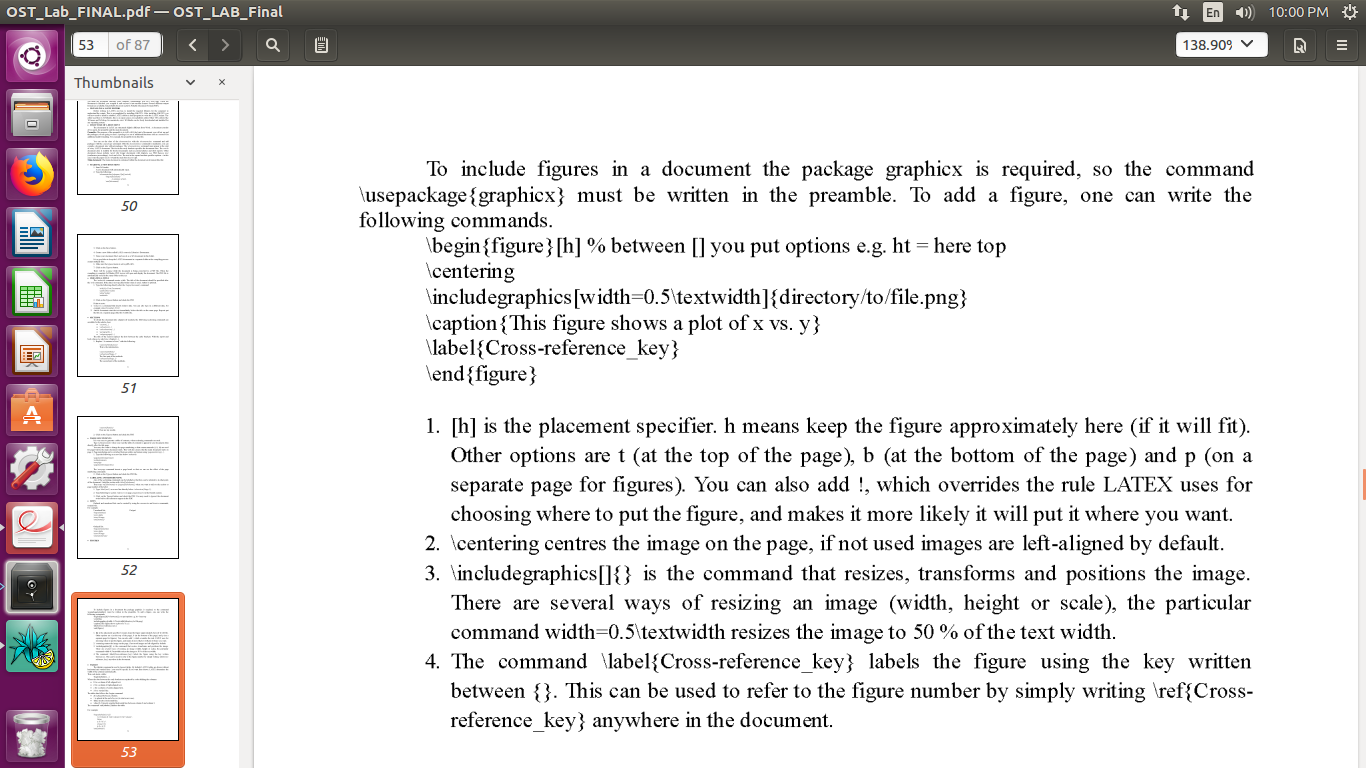
\includegraphics[width=0.5\textwidth]{figure.png}
\caption{Random Figure}
\label{crossref_key}
\end{figure}

\section{Table}
\begin{table}[h]
\centering
\begin{tabular}{|l|c|r|}
\hline
1st column&2nd column&3rd column\\
\hline
a & b & c\\
\cline{2-3}
1 & 2 & 3\\
\hline
\end{tabular}
\end{table}

\section{Multi-column}
\begin{table}[h]
\centering
\begin{tabular}{llc}
\hline%
\multicolumn{2}{c}{Sample} & Roughness\\
 & & (nm)\\
\hline%
A & Ring & 385\\
\cline{2-3}
 & Plate & 397\\
\hline
B & Ring & 376\\
\cline{2-3}
 & Plate & 390\\
\hline
\end{tabular}
\end{table}



\section{Results}
\ref{subsec1}
\newline
\ref{crossref_key}
\newline
End.

\end{document}
